\documentclass[aspectratio=169,12pt]{beamer}
\usetheme{metropolis}
\usepackage{graphicx}
\usepackage{booktabs}
\usepackage{tabularx}
\usepackage{tikz}
% \usepackage{fontspec}  % uncomment if using XeLaTeX/tectonic with system fonts
\usepackage{hyperref}

\definecolor{princeorange}{RGB}{255,143,0}
\definecolor{princeblack}{RGB}{0,0,0}
\definecolor{softblue}{RGB}{33,150,243}
\definecolor{softgreen}{RGB}{76,175,80}
\definecolor{softred}{RGB}{244,67,54}
\definecolor{lightgray}{RGB}{245,245,245}

\setbeamercolor{frametitle}{bg=princeblack,fg=white}
\setbeamercolor{progress bar}{fg=princeorange}
\setbeamercolor{alerted text}{fg=softred}

\title{Closing the Preprocessing Gap\\for Real-Time MindEye}
\subtitle{From Hours to Milliseconds on DGX Spark}
\author{Morgan G. Hough (m9h)}
\institute{Center17 ~|~ Orthogonal Research \& Education Lab (OREL) ~|~ Biopunk Lab ~|~ NeuroTechX}
\date{March 25, 2026}

\begin{document}

\maketitle

% ===================================================================
\section{Background}
% ===================================================================

\begin{frame}{MindEye2: Reconstructing Vision from Brain Activity}
\small
\begin{columns}[T]
\column{0.52\textwidth}
\textbf{Goal:} Reconstruct seen images from fMRI in real-time.

\vspace{0.3em}
\textbf{MindEye2} (Scotti et al., 2024):
\begin{itemize}\setlength\itemsep{0.1em}
    \item Pre-trained on NSD: 8 subjects, 30--40h of 7T fMRI
    \item Fine-tuned on Princeton \textbf{3T} sub-005 ($\sim$3h)
    \item GLMsingle betas $\rightarrow$ CLIP $\rightarrow$ SDXL unCLIP diffusion
\end{itemize}
\textcolor{softred}{\textbf{All RT benchmarks in this talk are 3T sub-005.}}

\vspace{0.3em}
\textbf{Model architecture} (frozen at inference):
\begin{enumerate}\setlength\itemsep{0.1em}
    \item \textbf{Ridge}: $(8627) \rightarrow (1024)$ hidden dim
    \item \textbf{MLP-Mixer}: $(1024) \rightarrow (256 \times 1664)$ OpenCLIP ViT-bigG-14
    \item \textbf{SDXL unCLIP}: CLIP $\rightarrow$ image
\end{enumerate}

\vspace{0.3em}
\textbf{Training pipeline:}\\
NSD 7T $\rightarrow$ fMRIPrep $\rightarrow$ GLMsingle $\rightarrow$ nsdgeneral betas $\rightarrow$ pre-train

\column{0.45\textwidth}
\begin{block}{Key Insight}
The model is frozen --- only the \textbf{input betas} change.\\[0.3em]
Better betas $\rightarrow$ better CLIP embeddings $\rightarrow$ better reconstructions.
\end{block}

\vspace{0.3em}
\begin{alertblock}{The Question}
Can we close the gap between the carefully processed \textbf{training betas} (fMRIPrep + GLMsingle) and the hastily computed \textbf{real-time betas} (simple GLM)?
\end{alertblock}
\end{columns}
\end{frame}

% -------------------------------------------------------------------

\begin{frame}{RT-Cloud MindEye: Real-Time at 3T}
\begin{columns}[T]
\column{0.55\textwidth}
\textbf{Princeton RT-Cloud project} (Iyer et al., 2026)\\
First real-time image reconstruction from fMRI.

\vspace{0.5em}
\textbf{Offline preparation:}
\begin{enumerate}\setlength\itemsep{0.1em}
    \item Collect 3 sessions of 3T data (sub-005)
    \item fMRIPrep: motion correction, registration,\\ distortion correction (all sessions aligned)
    \item GLMsingle: per-voxel HRF fitting, denoising,\\ridge regression $\rightarrow$ single-trial betas
    \item Voxel reliability $\rightarrow$ ``union mask'' (8627 voxels)
    \item Fine-tune MindEye2 on masked betas
\end{enumerate}

\vspace{0.3em}
\textbf{Real-time session (ses-06):}
\begin{enumerate}\setlength\itemsep{0.1em}
    \setcounter{enumi}{4}
    \item Stream DICOM volumes via RT-Cloud (TR=1.5s)
    \item Motion correct + register to ses-01 reference
    \item Fit growing-window GLM $\rightarrow$ single-trial beta
    \item Z-score beta over running history
    \item MindEye forward pass $\rightarrow$ reconstruction
    \item Display to participant (PsychoPy)
\end{enumerate}

\column{0.42\textwidth}
\begin{alertblock}{The Problem}
The \textbf{training betas} went through fMRIPrep + GLMsingle (hours of processing).\\[0.3em]
The \textbf{real-time betas} use a simple nilearn GLM.\\[0.3em]
This \textbf{train/test mismatch} degrades reconstruction quality.
\end{alertblock}
\end{columns}
\end{frame}

% -------------------------------------------------------------------

\begin{frame}{The Preprocessing Gap: Offline vs Real-Time}
\footnotesize
\centering
\begin{tabular}{@{}l l l l@{}}
\toprule
\textbf{Stage} & \textbf{Offline (training)} & \textbf{Real-Time (current)} & \textbf{Gap?} \\
\midrule
Brain extraction & SynthStrip & Pre-computed mask & --- \\
Tissue segmentation & FreeSurfer & --- & minor \\
Surface recon & recon-all (6h) & --- & minor \\
Func$\rightarrow$Anat reg. & bbregister & FLIRT (1$\times$) & minor \\
Motion correction & MCFLIRT & MCFLIRT (CPU) & --- \\
Distortion correction & Fieldmaps & --- & minor \\
Slice timing & Fourier interp & --- & minor \\
\textbf{Confound regression} & \textbf{CompCor (WM/CSF)} & \textcolor{softred}{\textbf{None}} & \textcolor{softred}{\textbf{MAJOR}} \\
\midrule
\textbf{HRF model} & \textbf{Per-voxel (20 library)} & \textcolor{softred}{\textbf{Single Glover}} & \textcolor{softred}{\textbf{MAJOR}} \\
\textbf{Noise regression} & \textbf{GLMdenoise} & \textcolor{softred}{\textbf{None}} & \textcolor{softred}{\textbf{MAJOR}} \\
\textbf{Regularization} & \textbf{Ridge (cross-val)} & \textcolor{softred}{\textbf{None}} & \textcolor{softred}{\textbf{MAJOR}} \\
\bottomrule
\end{tabular}

\vspace{0.8em}
\normalsize
\textcolor{softred}{\textbf{Four critical stages missing}} in real-time $\rightarrow$ train/test mismatch degrades reconstruction quality.\\
All addressable with JAX/GPU acceleration at $<$100ms total.
\end{frame}

% ===================================================================
\section{Proposed Pipeline}
% ===================================================================

\begin{frame}{Proposed RT Pipeline: Closing the Gap}
\centering
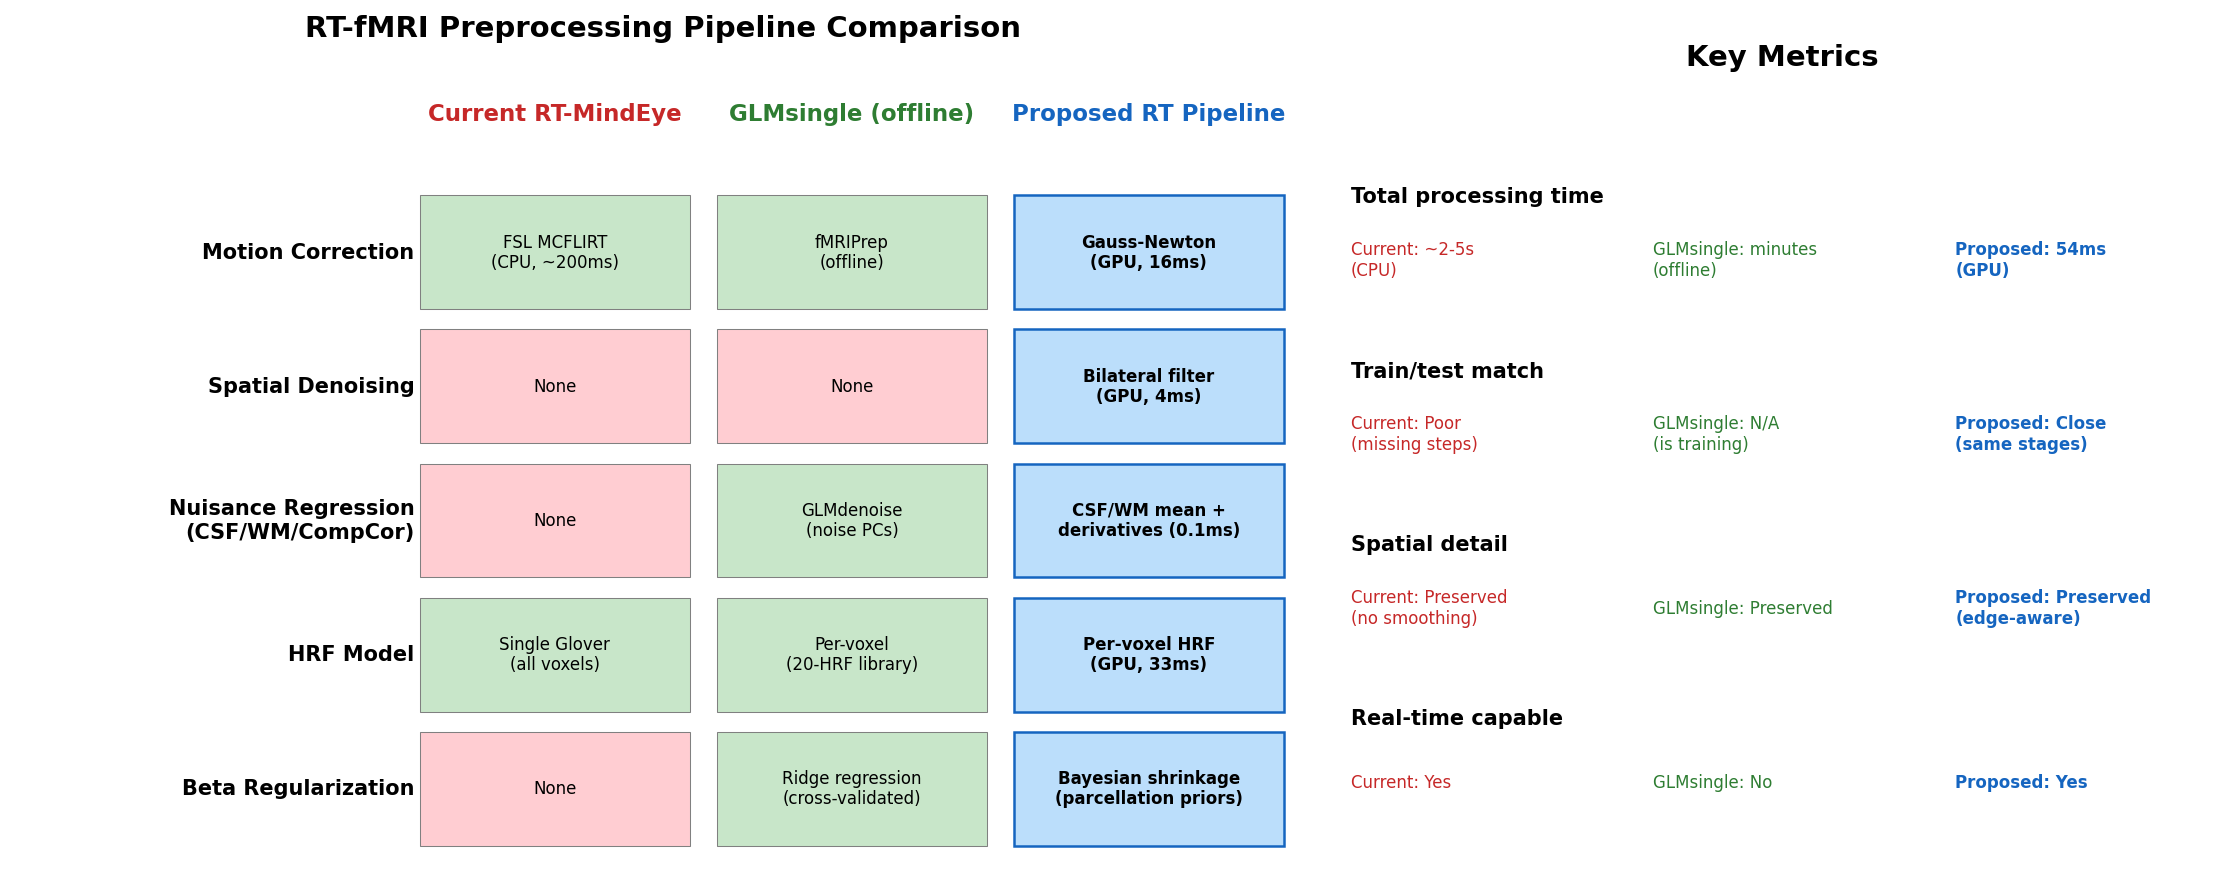
\includegraphics[width=\textwidth]{pipeline_comparison.png}
\end{frame}

% -------------------------------------------------------------------

\begin{frame}{From Hours to Milliseconds}
\centering
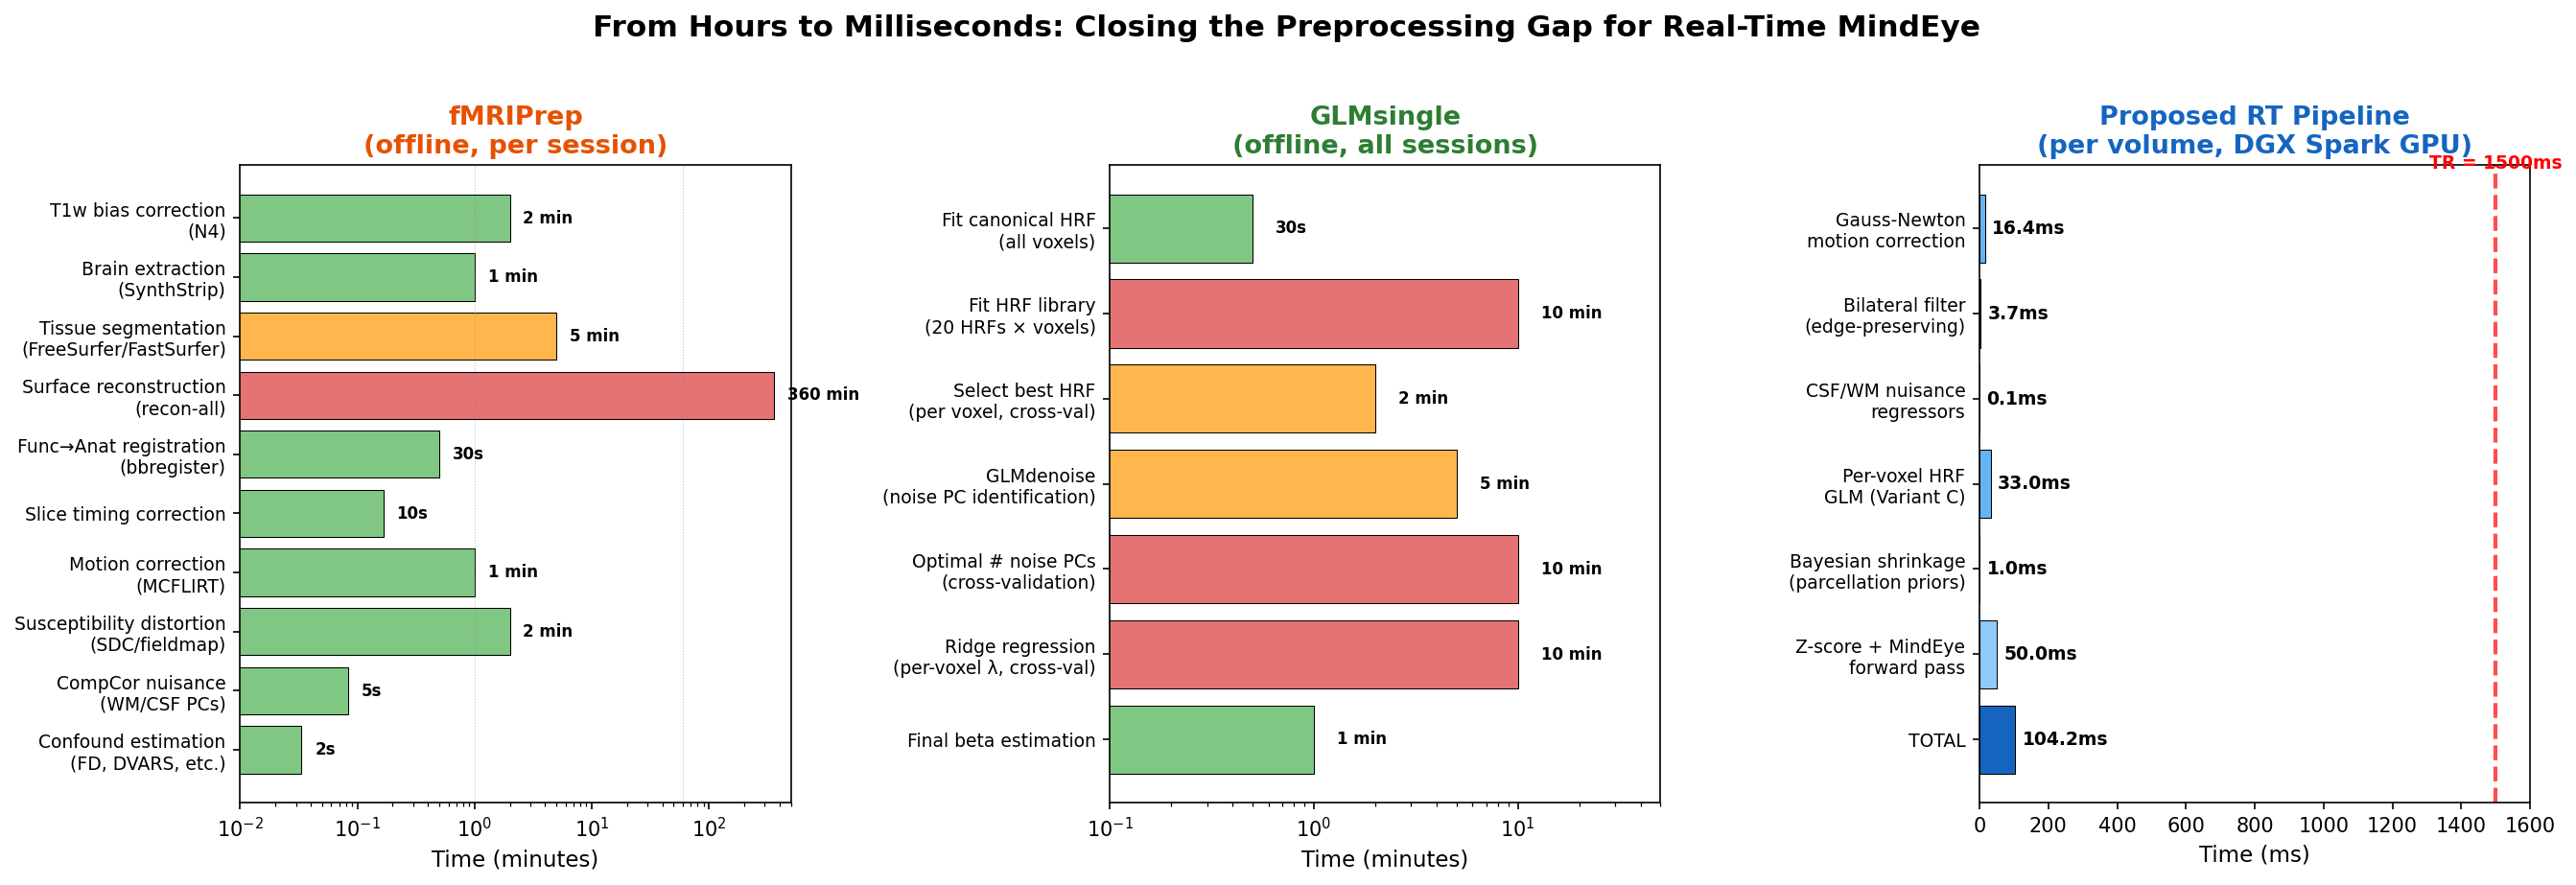
\includegraphics[width=\textwidth]{timing_budget.png}
\end{frame}

% ===================================================================
\section{Variant Comparison}
% ===================================================================

\begin{frame}{Preprocessing Variant Benchmark}
\centering
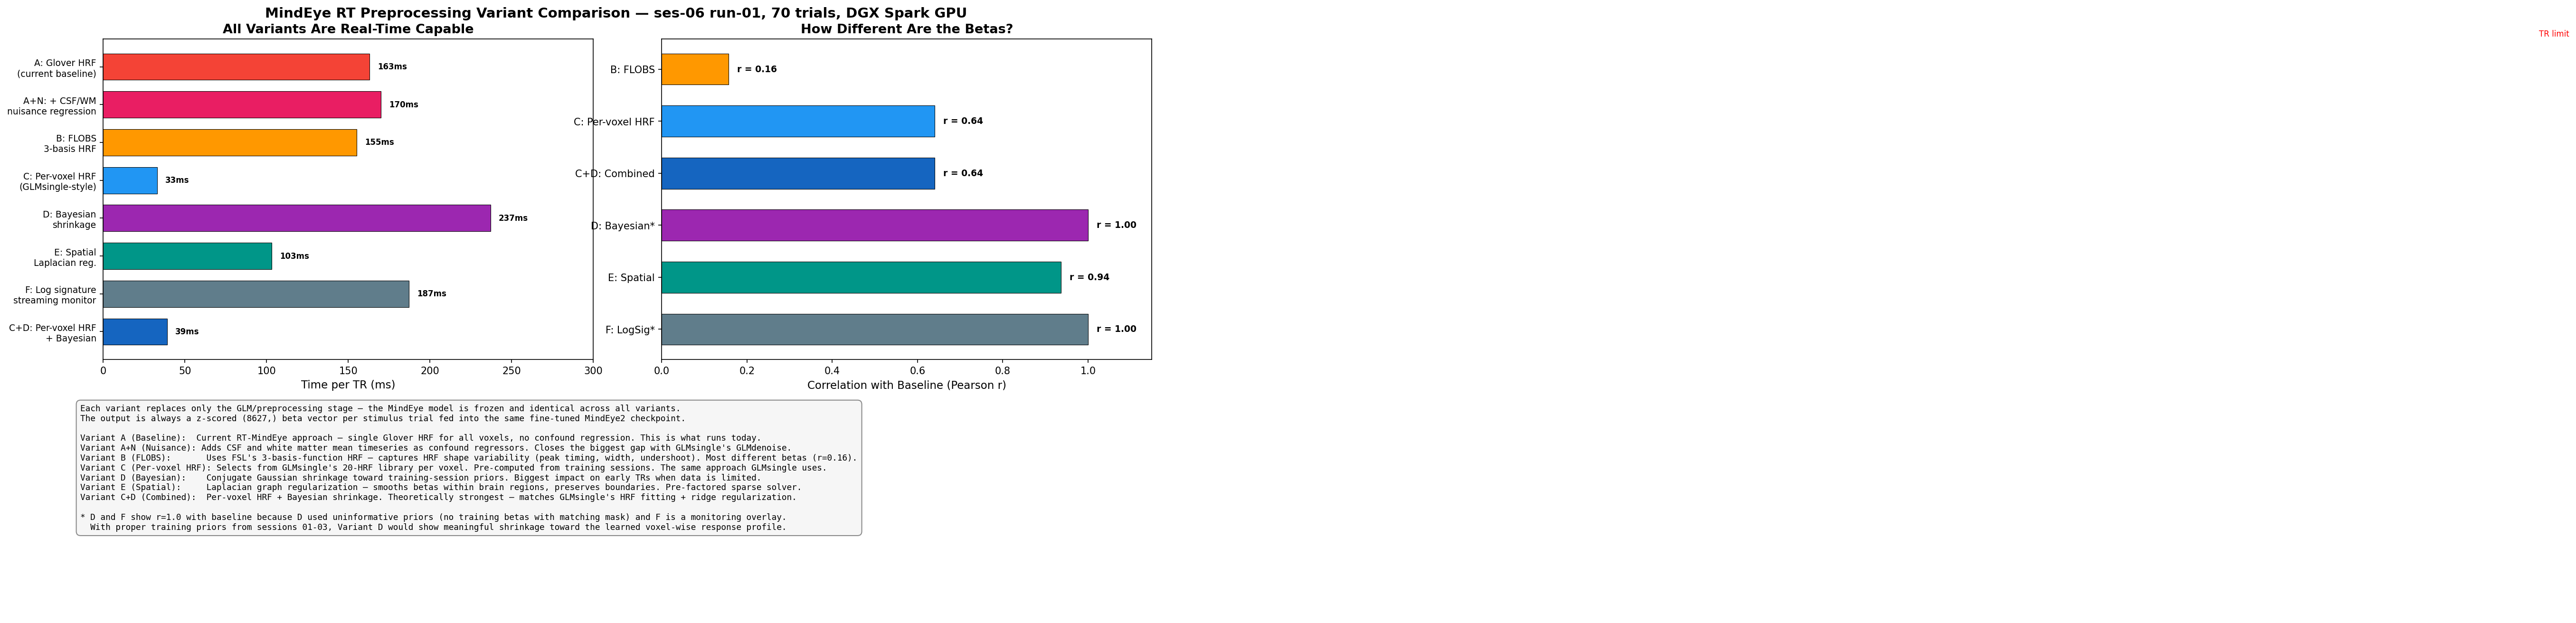
\includegraphics[width=\textwidth]{variant_benchmark_explained.png}
\end{frame}

% ===================================================================
\section{Dimensionality Estimation}
% ===================================================================

\begin{frame}{Eigenspectrum: 3T Single-Subject vs 7T Multi-Subject}
\centering
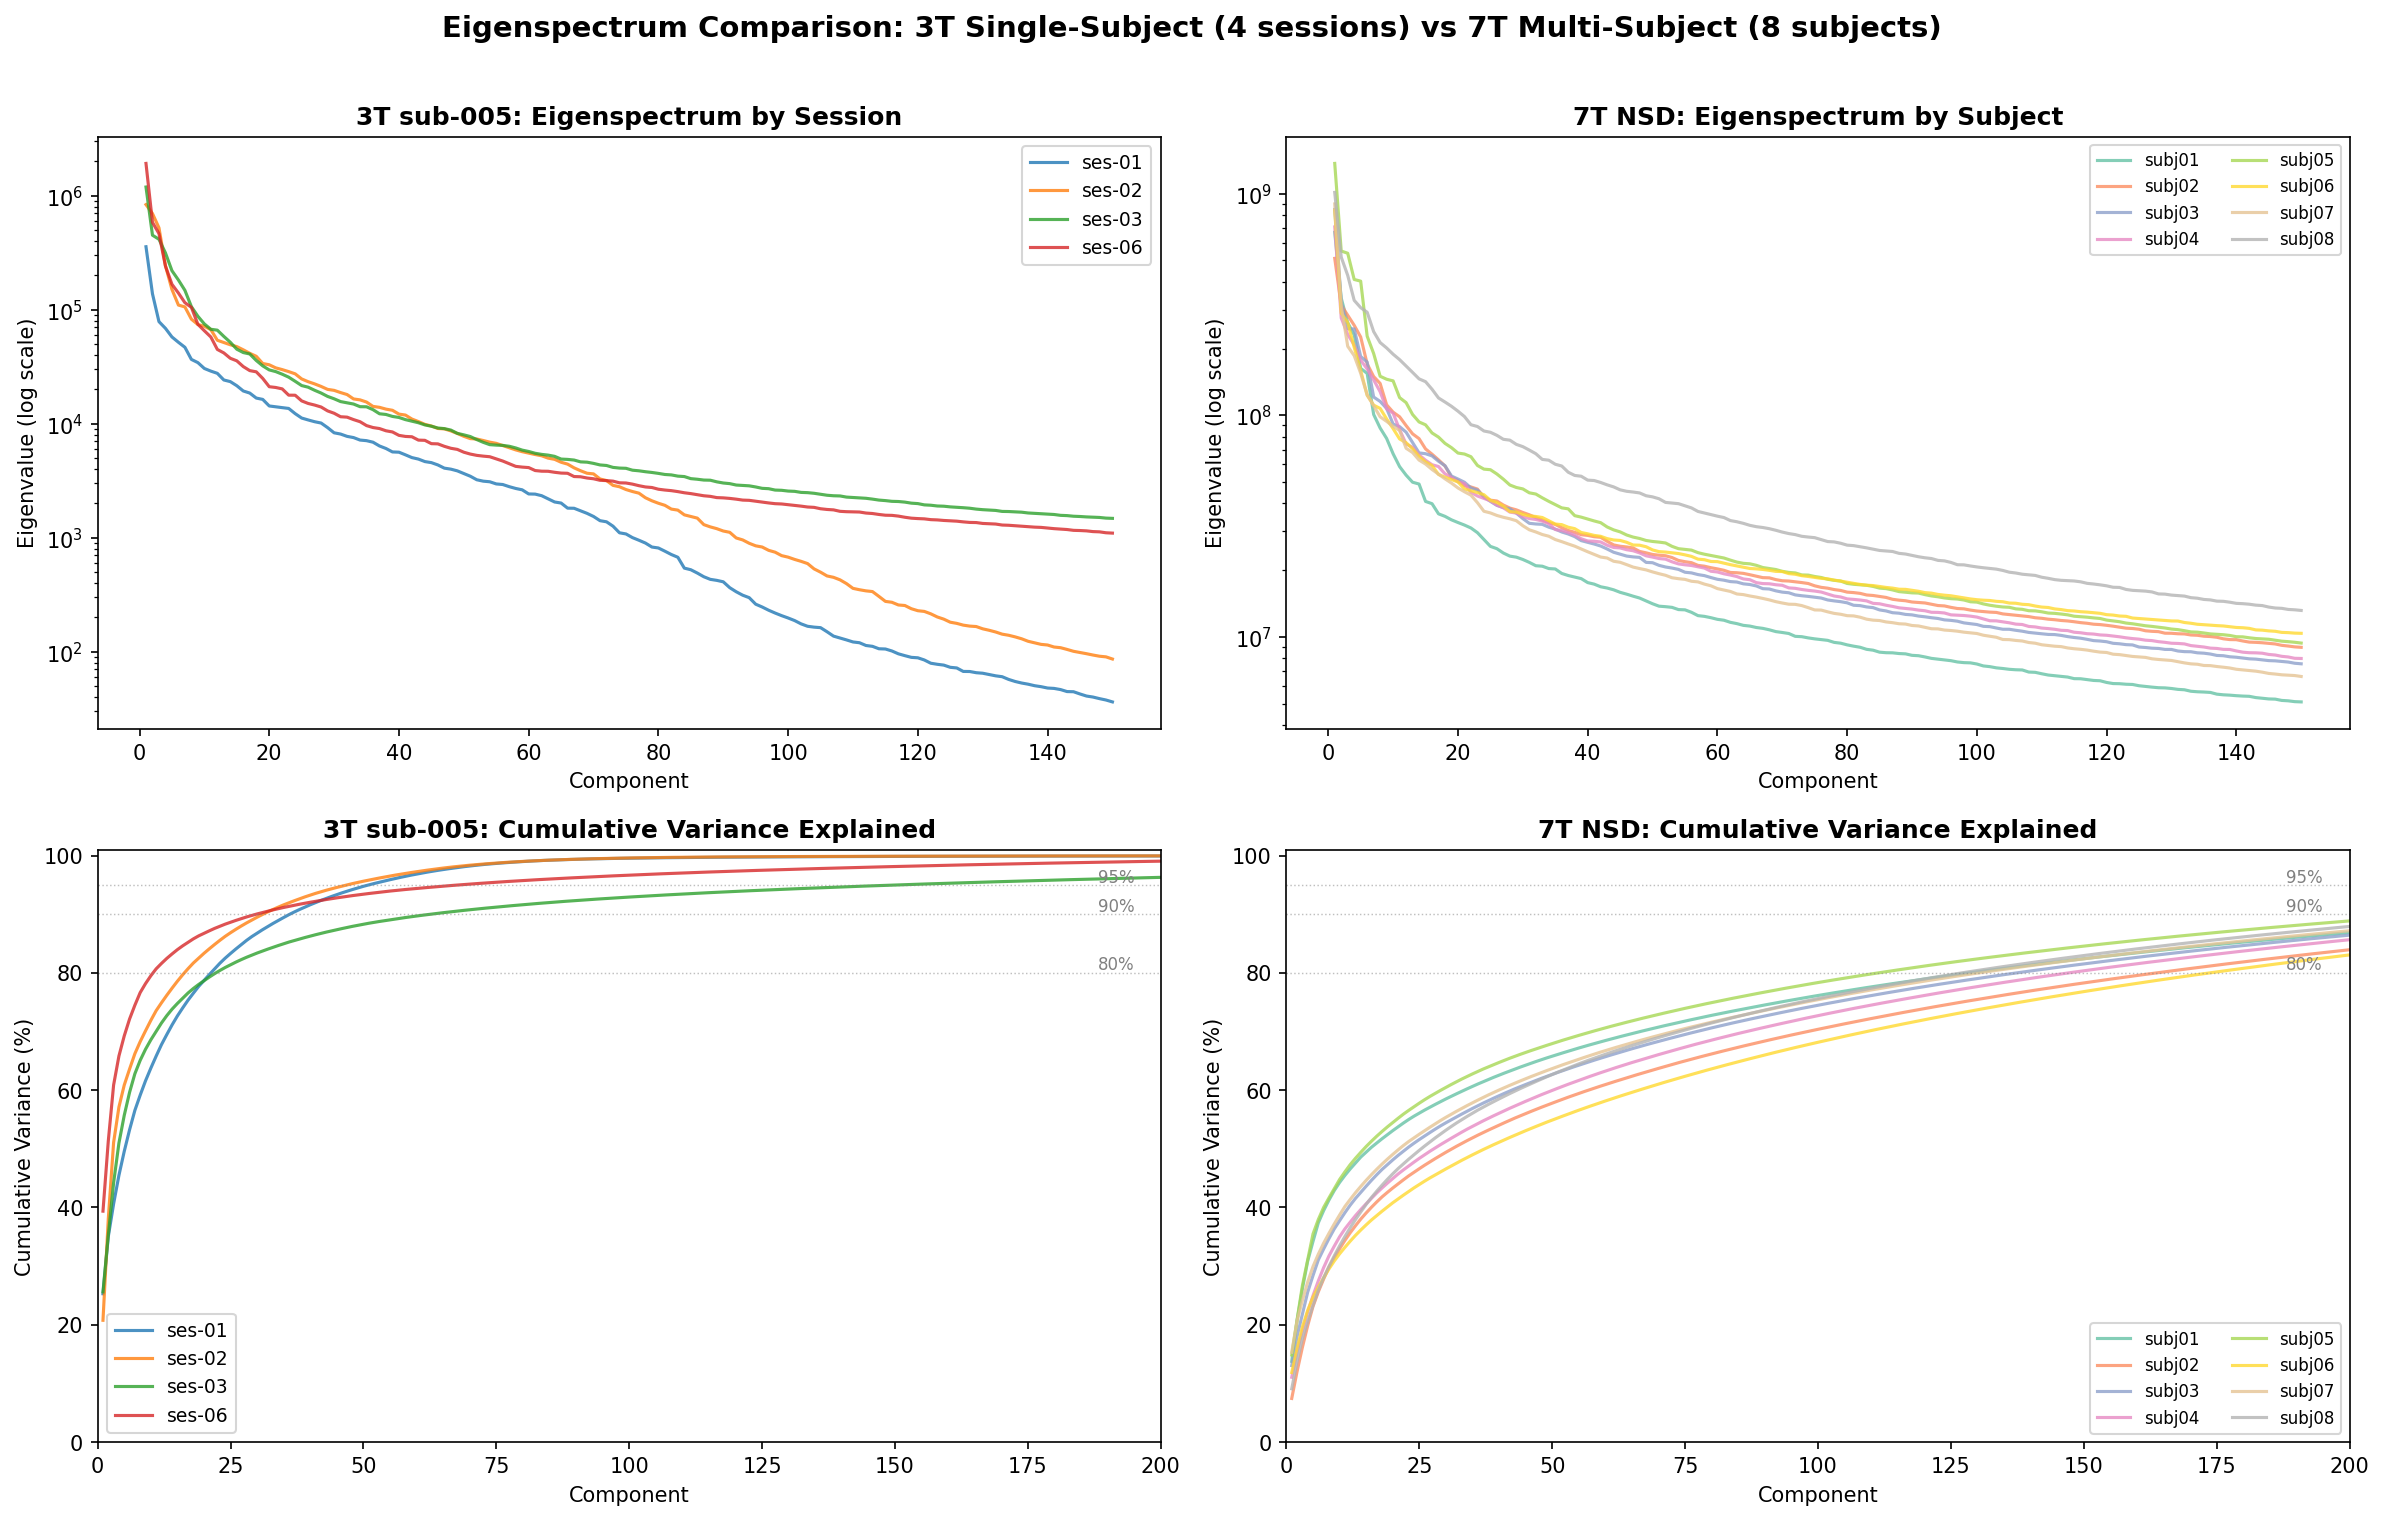
\includegraphics[width=\textwidth]{eigenspectrum_3t_vs_7t.png}
\end{frame}

% -------------------------------------------------------------------

\begin{frame}{Dimensionality Across 8 NSD Subjects}
\centering
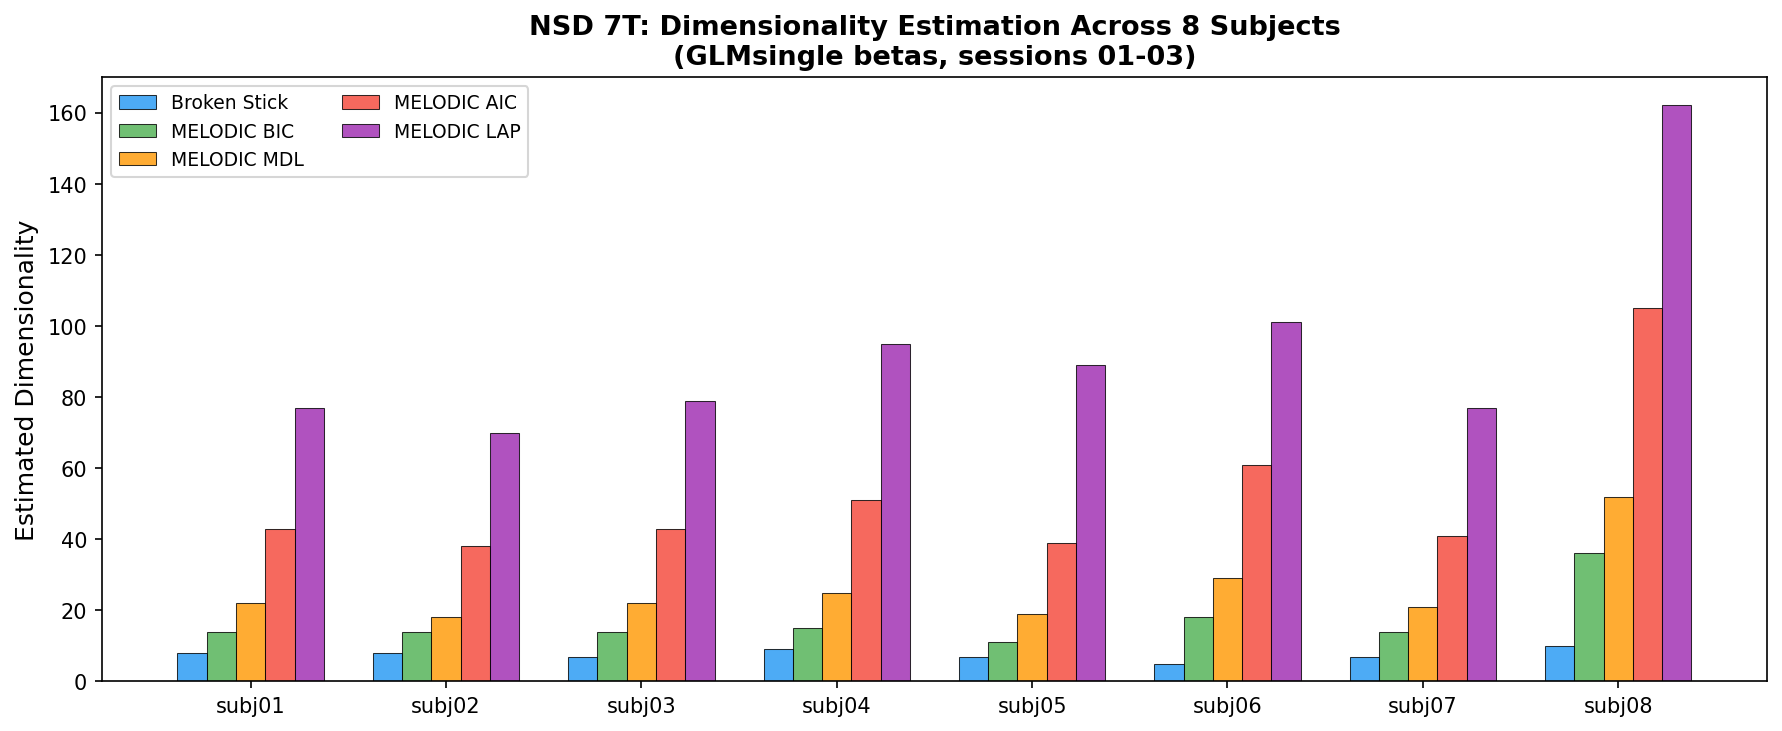
\includegraphics[width=0.85\textwidth]{nsd_dimest_presentation.png}

\vspace{0.5em}
\small
\begin{columns}[T]
\column{0.48\textwidth}
\textbf{NSD (7T, 8 subjects):}
\begin{itemize}
    \item BIC most consistent: 11--18 across 7/8 subjects
    \item 7T data needs $>$200 PCs for 80\% variance
    \item subj08 is a clear outlier across all methods
\end{itemize}

\column{0.48\textwidth}
\textbf{Princeton sub-005 (3T, 4 sessions):}
\begin{itemize}
    \item Conservative (broken stick): 14--24 per session
    \item Liberal (parallel analysis): 30--67
    \item 3T needs only 22--45 PCs for 80\% variance
    \item MELODIC BIC: 21--42 per session
\end{itemize}
\end{columns}
\end{frame}

% ===================================================================
\section{Anatomy-Informed Processing}
% ===================================================================

\begin{frame}{FastSurfer Integration: In-Session Anatomy}
\centering
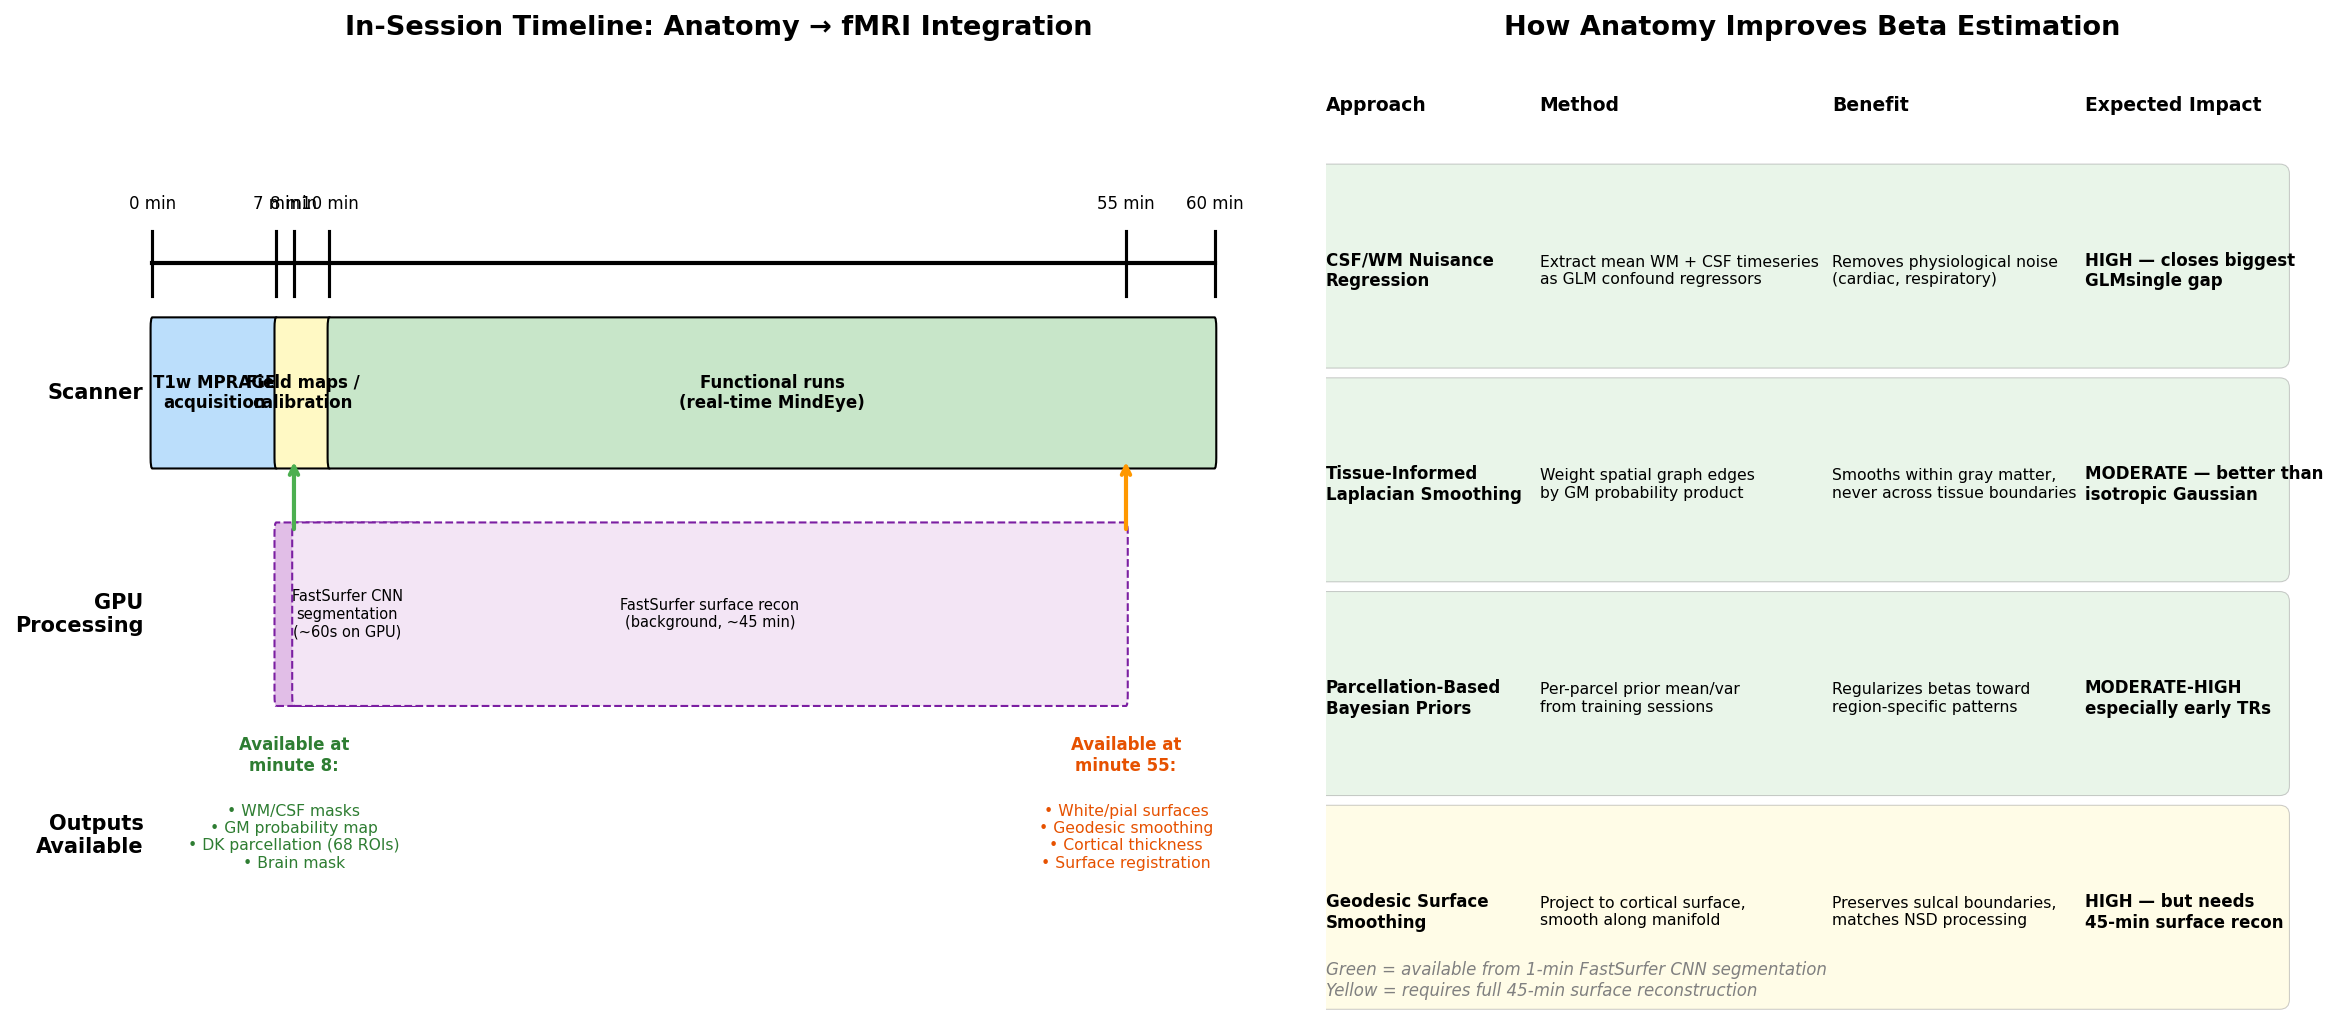
\includegraphics[width=\textwidth]{anatomy_integration.png}
\end{frame}

% ===================================================================
\section{New Spatial Processing}
% ===================================================================

\begin{frame}{Edge-Preserving Denoising \& GPU Motion Correction}
\centering
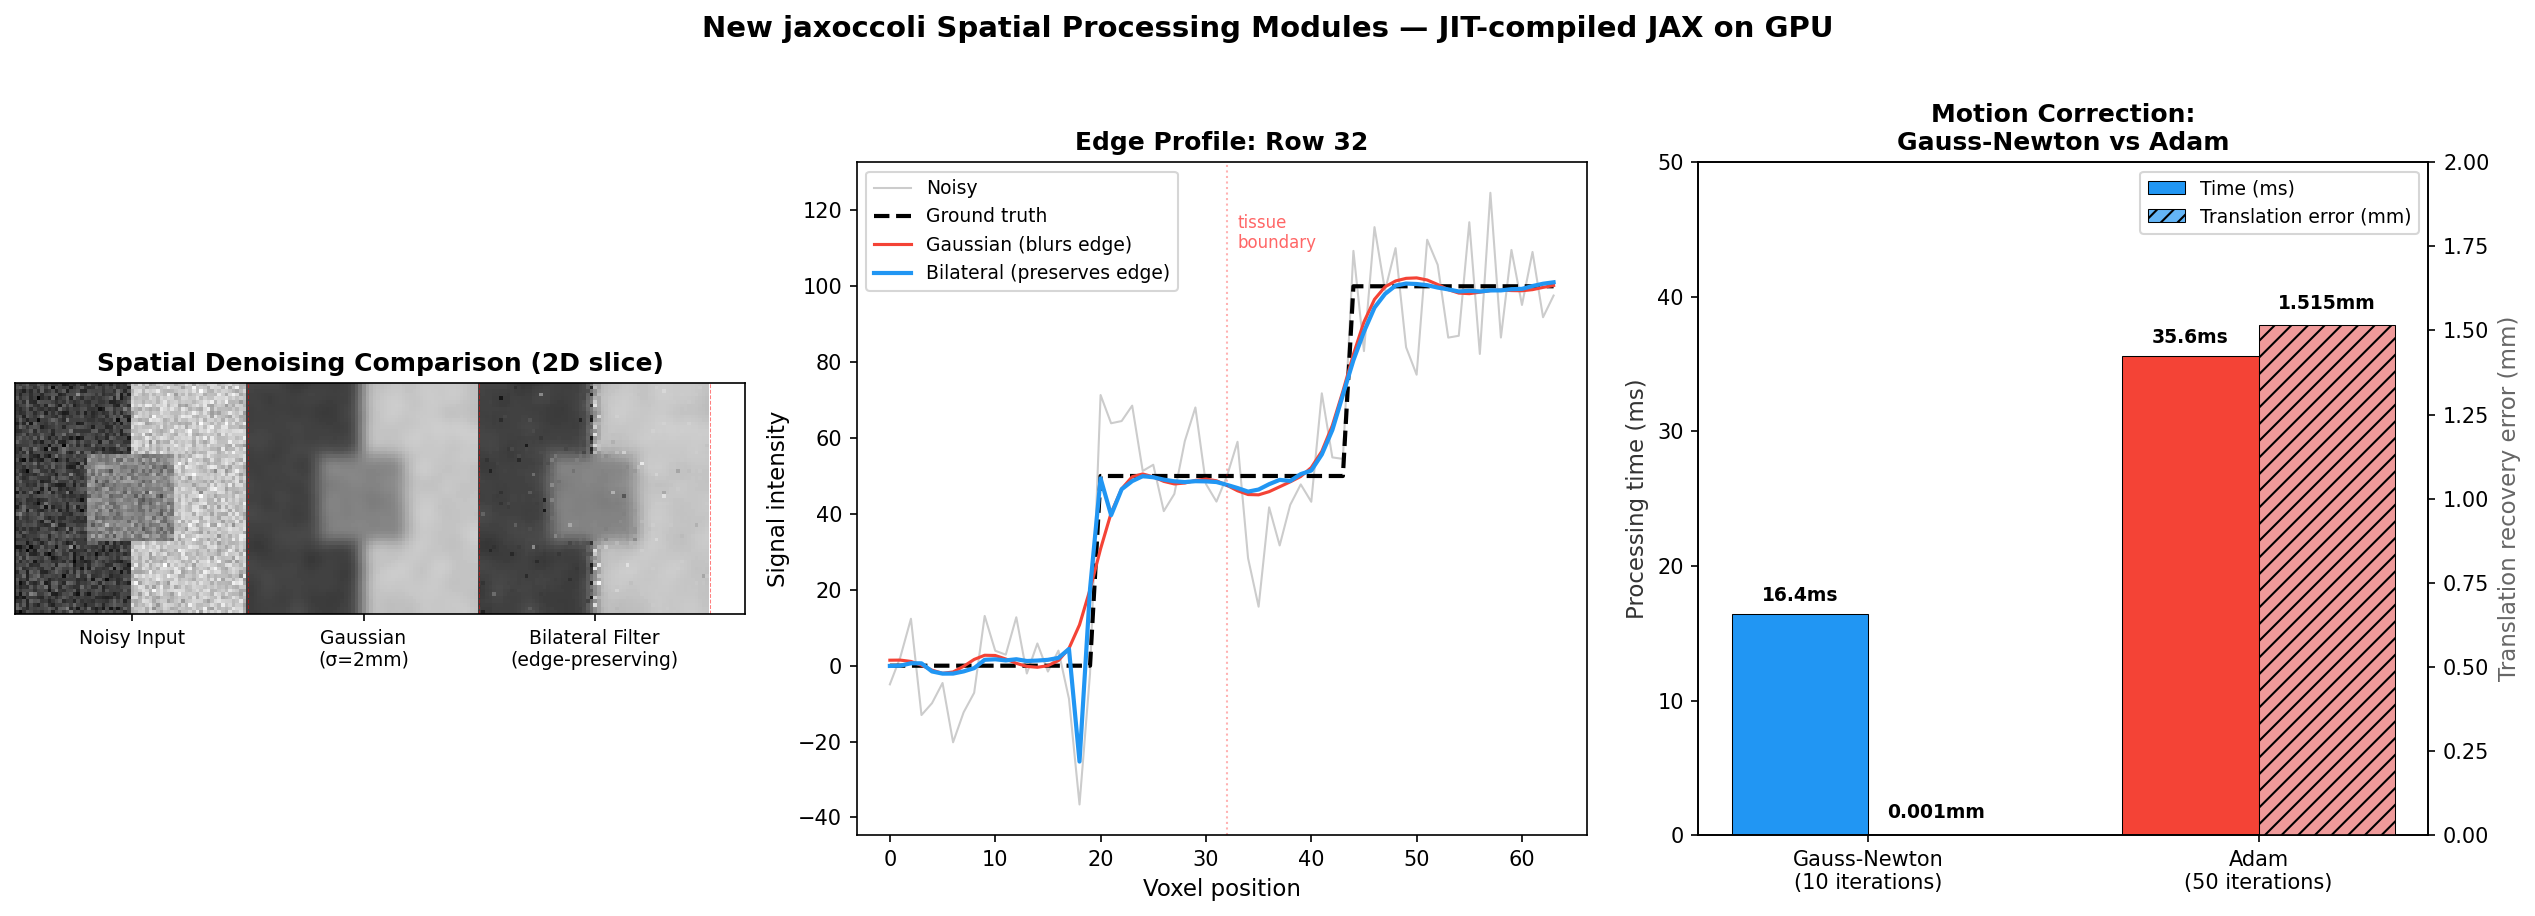
\includegraphics[width=\textwidth]{spatial_processing_new.png}
\end{frame}

% ===================================================================
\section{Summary}
% ===================================================================

\begin{frame}{Summary \& Next Steps}
\begin{columns}[T]
\column{0.48\textwidth}
\begin{block}{What We Built}
\begin{itemize}
    \item 8 preprocessing variants, all $<$1.5s/TR on GPU
    \item Per-voxel HRF (GLMsingle-style): \textbf{33ms}
    \item Bilateral filter: \textbf{3.7ms}
    \item Gauss-Newton MC: \textbf{16ms}, 2.2$\times$ faster than Adam
    \item CSF/WM nuisance regression: \textbf{0.1ms}
    \item Sparse spatial regularization: \textbf{103ms} (was 11s)
    \item Full proposed pipeline: \textbf{$\sim$54ms total}
\end{itemize}
\end{block}

\column{0.48\textwidth}
\begin{block}{Next Steps}
\begin{enumerate}
    \item Run MindEye inference on variant betas\\(requires NGC PyTorch container)
    \item Compare reconstruction quality:\\CLIP retrieval accuracy, SSIM
    \item Integrate FastSurfer CNN ($\sim$60s)\\for anatomy-informed priors
    \item NORDIC PCA denoising on sliding window
    \item Incremental Patch2Self adaptation
    \item Containerize: Dockerfile ready
\end{enumerate}
\end{block}
\end{columns}

\vspace{0.5em}
\centering
\small
All code at \texttt{hippy-feat/scripts/rt\_glm\_variants.py} ~|~ Results on NFS at \texttt{/data/derivatives/mindeye\_variants/}\\
85 passing tests ~|~ NSD dimensionality results across 8 subjects ~|~ MELODIC reports generated
\end{frame}

\end{document}
